\chapter{Introduzione}
%\myChapter{Introduzione}

%-------------------	Descrizione del problema -------------------------------
Ipotesi: \textit{� possibile costruire un sistema intelligente e portatile in grado di riconoscere (classificare) e analizzare i movimenti di un individuo e di fornirne in linea (vedi Appendice \ref{sec:real_time_sys}) informazioni a riguardo}.\\

Il problema del riconoscimento (classificazione) di una generica attivit� motoria umana � irrisolto ed estremamente complesso visto il numero esorbitante di parametri coinvolti.
In questo lavoro viene affrontata l'analisi di una singola attivit� nota: la deambulazione entro un intervallo di velocit� e pendenza del terreno.

Nello specifico il problema � quello dell'individuazione in linea delle tempistiche di eventi che costituiscono una deambulazione normale come studiato dalla Chinesiologia (vedi Capitolo \ref{cap:chinesiologia}). Tale problema � noto come \emph{problema della segmentazione automatica ed in linea della deambulazione umana}.\\

%------------------  Motivazioni del problema Perch� si pone?--------------------------------
La soluzione del problema della segmentazione avrebbe risvolti immediati nella Medicina riabilitativa per la diagnosi e/o assistenza a persone con problemi di deambulazione, nella Robotica e Computer Grafica per la emulazione/simulazione della deambulazione umana, nel mondo dello sport agonistico per l'apprendimento di specifiche tecniche motorie.\\

%---------------------� gia stato affrontato? 
Il problema della segmentazione � stato ampiamente affrontato nella letteratura scientifica (letteratura biomedica, biomeccanica, ingegneria medica) con svariate combinazioni di materiali e metodi. 

Per quanto riguarda i materiali, sono state proposte soluzioni basate sull'osservazione diretta di un fisiatra; basate sulla stereofotogrammetria, sistemi di telecamere ad emissione di luce infrarossa e marcatori riflettenti; basate su strumenti inerziali, sensori fisici: accelerometri, giroscopi, elettromagnetometri. 
\begin{figure}
	\centering
	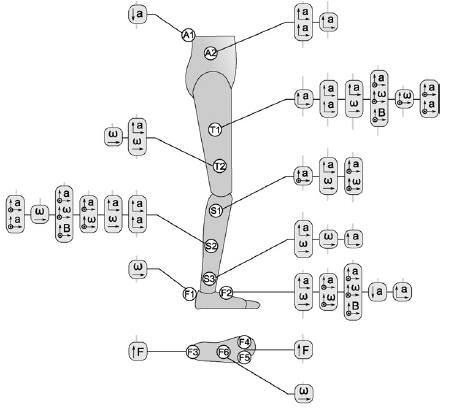
\includegraphics[width=1\textwidth]{imgs/sensorOnBodyLocations.jpg}
	\caption{Schema riassuntivo dei posizionamenti di diversi sensori su diverse parti del corpo, usati in letteratura. Nella Figura, $a$ rappresenta un accelerometro, $\omega$ rappresenta un giroscopio, $B$ rappresenta un magnetometro. Le frecce accanto alle lettere rappresentano le dimensioni dei rispettivi sensori, quindi una frecce sotto un simbolo significa che il sensore � monoassiale, due significa biassiale e tre (la terza freccia � uscente, quindi rappresentata come un cerchio con un punto al suo centro) triassiale. Le `capsule` grigie che racchiudono uno o pi� sensori sono dette Unit� Sensoriali. Le lettere A (\textit{abdomen}, addome), T (\textit{thigh}, coscia), S (\textit{shank}, stinco) ed F (\textit{foot}, piede) rappresentano le parti del corpo sui quali si trovano. 
	 Figura adattata da \cite{gait_event_detection_analysis}}
	\label{fig:sensorOnBodyLocations}
\end{figure}
Questi ultimi sono stati usati in diverse combinazioni, numero e disposizione sul corpo (vedi Figura \ref{fig:sensorOnBodyLocations}).\\ 

Per quanto riguarda i metodi, sono state proposte soluzioni 
di tipo cinematico basato sullo studio delle forze che agiscono sul corpo nella deambulazione; di tipo analitico (studio di funzioni e curve) basato sull'analisi funzionale dei segnali di sensori inerziali; 
di tipo modellistico basate sugli Automi a Stati Finiti per lo studio di sequenze temporali; 
pi� di recente di tipo informatico-statistico basati sull'Apprendimento Automatico (Reti Neurali, Logica Fuzzy) per la capacit� di astrarre sulle variazioni dei singoli individui \cite{gait_event_detection_analysis}.

% -------------------------------� stato gia stato risolto? 
Nonostante il vasto numero di lavori, non � ancora stata data una soluzione soddisfacente al problema. 
Tutti i metodi proposti peccano di dipendenza dai soggetti per i quali quali vengono creati, vale a dire che variando questi ultimi, variano le prestazioni dei metodi. Questo � indice di bassa capacit� di generalizzazione dei metodi.\\

%------------------------- Come voglio affrontare il problema? 
La scelta dell'utilizzo delle HMM � giustificata dai seguenti motivi. 
Le HMM (vedi Appendice \ref{cap:hmm}) sono uno strumento stocastico di riconoscimento di schemi (\textit{Stochastic Pattern Recognition}) usato in campi come il riconoscimento vocale \cite{tutorial_hmm_application_speech_recognition} e lo studio della visione artificiale per il riconoscimento gestuale \cite{HMM_gesture_recognition}. Uno studio dimostra il potenziale delle HMM per la segmentazione della deambulazione equina \cite{stride_segmentation_technique_hmm}. \\

Inoltre vi sono studi che usano le HMM come struttura gerarchica per affrontare il problema della classificazione di attivit� umane \cite{human_physical_activity_classification_ml, spatio_temporal_params_gait_gyr}. Per sviluppi futuri, del lavoro qui presentato, nella direzione della risoluzione del problema della classificazione, gli studi citati sono a favore dell'utilizzo delle HMM.
